\documentclass[draft]{agujournal2018}
\usepackage{apacite}

\usepackage{lineno}
\usepackage{amsmath}
\usepackage{xcolor}



\begin{document}
\title{%
  Deformations from Sea-Ice Tracker Data \\
  \large Beatrice Duval}


%\title{}

The algorithm presented in this document aims at computing arctic sea-ice deformations from ice-tracker data (Sentinel-1 and RCM). The algorithm takes as input a list of tracked features with their starting and ending Latitude/Longitude positions, and produces a deformations dataset.

The RIOPS grid is used throughout the execution of this algorithm. More specifically, we use a cropped version of the RIOPS grid that defines our region of interest (Fig. \ref{grid}). Additionnaly, we add to the grid a distance to land matrix, a land-sea mask, and a matrix of X/Y tracer points in the Azimuthal Equidistant projection.  

\begin{figure}[h]
 \begin{center}
   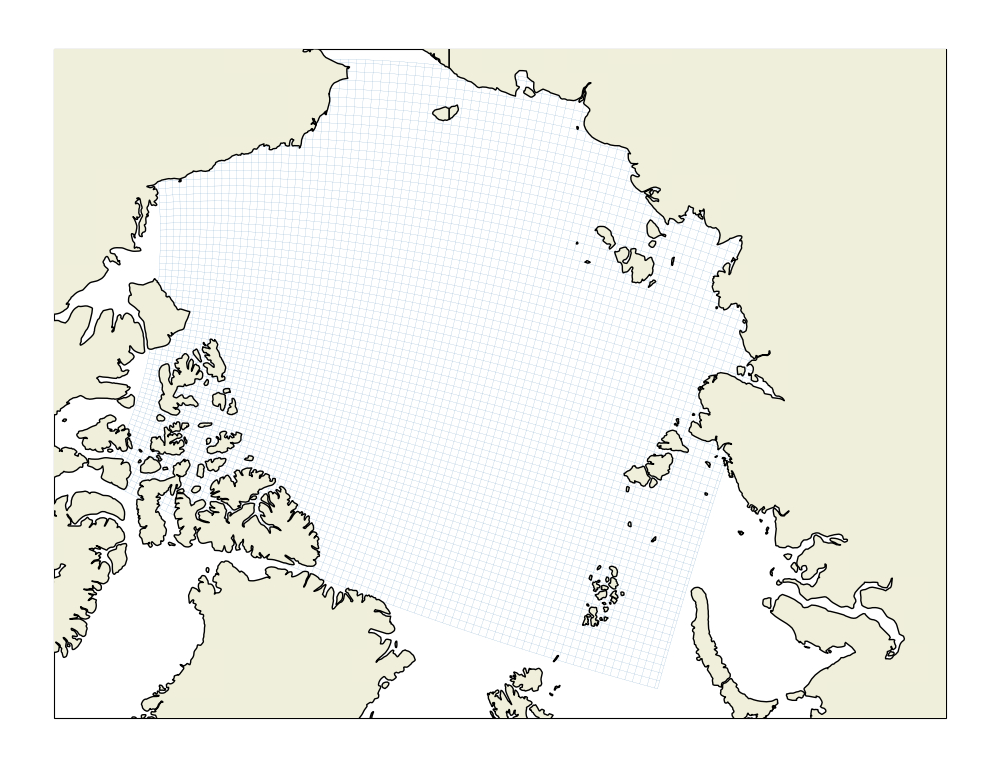
\includegraphics[scale=.4]{figures/grid_lines.png}
 \end{center}
 \caption{A cropped RIOPS grid is used to define the region of interest, as well as to define local Cartesian coordinate systems.}
 \label{grid}
\end{figure}

The input data is processed in 3 steps. First, a Delaunay triangulation is performed on the input data. These results are then converted from Latitude/Longitude to X/Y Cartesian coordinates in a local Cartesian coordinate system based on the RIOPS grid. Finally, deformations are computed. The following describes these steps.

\section{Performing a Delaunay Triangulation}

First, a Delaunay triangulation algorithm \textit{scipy.spatial.Delaunay} is used to organize the tracked features into triangular arrays. 

\section{Conversion to Cartesian Coordinates}

For every triangle found in the previous step, we want to convert each vertex's starting and ending positions from Latitude/Longitude to X/Y coordinates. In order to avoid conversion errors, we define a local Cartesian coordinate system for each triangle using the RIOPS grid (Fig. \ref{axes-locaux}). That is, for each triangle:

\begin{itemize}
    \item We find the RIOPS grid tracer point nearest to the triangle center (e.g. point T in Fig. \ref{axes-locaux}), and define a ``local cell'' based on the neighbouring speed points (A, B, C and D in Fig. \ref{axes-locaux}).
    % Region of interest: rejection of points is done here
    \item The origin is defined at the Southwest node (C in Fig. \ref{axes-locaux}) and the x and y axis are defined from the southern and eastern cell vertices respectively (sea blue arrows in Fig. \ref{axes-locaux}).
    
    \item Using haversine, we compute the distance between the origin and the nodes B and D, such that we can express their position in the local Cartesian coordinate system: B $ = (0, b)$ and D $=(d,0)$.
\end{itemize}

\begin{figure}[h]
 \begin{center}
   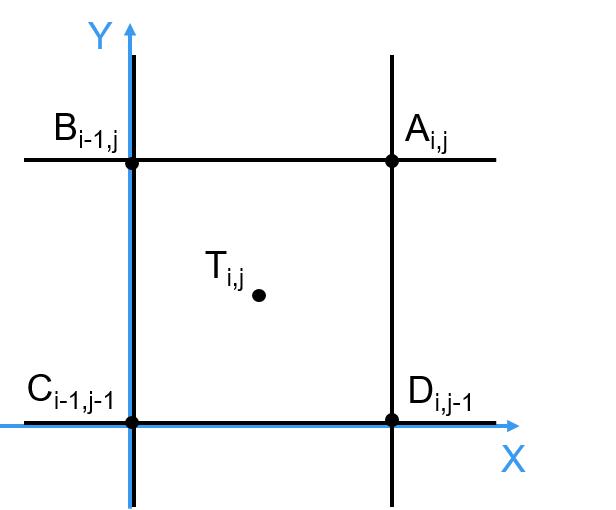
\includegraphics[scale=.6]{figures/localCS.png}
 \end{center}
 \caption{Given a tracer point at (i, j), the origin is defined at the speed point (i-1, j-1), and the x and y-axes are defined by the local grid cell.}
 \label{axes-locaux}
\end{figure}


We now find the starting and ending positions of each triangle vertex in the local Cartesian coordinate system via triangulation (Fig. \ref{triangulation}):

\begin{itemize}
    
    \item Using haversine, we find the distances $a_1, a_2$ and $a_3$ between the vertex P and the nodes B, C and D. 
    
    \item We now have 3 circles centered at B, C and D and with $a_1, a_2$ and $a_3$ radii, respectively. The X/Y position of the vertex P corresponds to the intersection of the 3 circles. More specifically,
    
\begin{align*}
    x = \frac{a_2^2-a_3^2+d^2}{2d} \;\; \text{and} \;\;
    y = \frac{a_2^2-a_1^2+b^2}{2b}.
\end{align*}
  
\end{itemize}


\subsection{Rejection of Data}

If the distance between a triangle's center point and its nearest grid tracer point is greater than 10 km, we reject that data set since it is not within the region of interest defined by the RIOPS grid (neighboring tracer points are at most 8 km apart). Moreover, we reject a triangle if its tracer point's distance to land is 0, that is if the triangle is located on land. Lastly, once we have the triangle's vertex positions in Cartesian coordinates, we compute its angles and reject it if it has an angle of less than 10 degrees. 

Otherwise, we proceed to the next step, that is computing deformations.

\begin{figure}[h]
 \begin{center}
   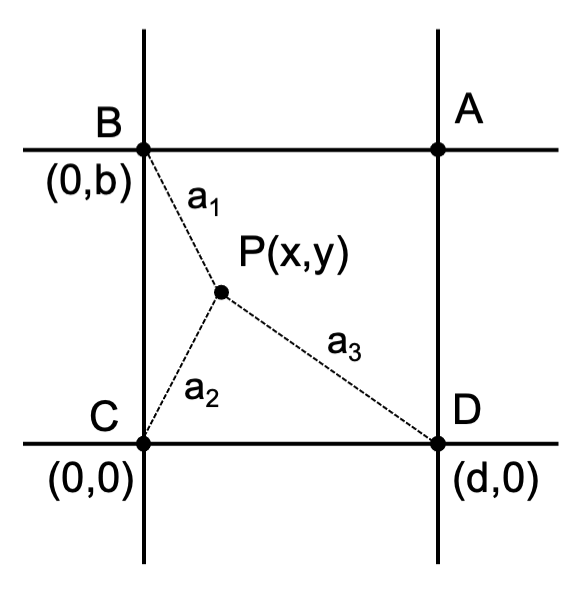
\includegraphics[scale=.6]{figures/triangulation.png}
 \end{center}
 \caption{ We convert the triangle vertex positions from Latitude/Longitude to X/Y coordinates in a local Cartesian coordinate system via triangulation.}
 \label{triangulation}
\end{figure}

\section{Computing Deformations}

We compute deformations for every triangle using X/Y coordinates in a local Cartesian coordinate system as computed in the previous step and following \textit{Bouchat et al. (2020)}.


\end{document}